\documentclass[a4paper,12pt]{article}

\usepackage{graphicx}
\usepackage{caption}
\usepackage{subcaption}
\usepackage{tikz}
\usepackage{pgf}
\usepackage{amsmath}
\usepackage{amssymb}
\usetikzlibrary{arrows.meta}
\usepackage[utf8]{inputenc}
\usepackage[english,greek]{babel}
\usepackage{hyperref}

\title{Εργασία Μέρος Β - Θεωρία Εκτίμησης και Ανίχνευσης \\[0.5cm] Ομάδα 29}
\author{Αριστείδης Δασκαλόπουλος (ΑΕΜ: 10640) \\ Ρουσομάνης Γεώργιος (ΑΕΜ: 10703)}
\date{Ιούνιος 2025}

\begin{document}

\maketitle

\section*{Εισαγωγή}

Σκοπός της παρούσας εργασίας είναι η αποθορυβοποίηση πολυκαναλικών ΗΕΓ σημάτων $y[k] \in \mathbb{R}^N$, τα οποία περιέχουν παρεμβολές λόγω ανοιγοκλεισίματος των ματιών. Το σήμα μοντελοποιείται ως
\[
\mathbf{y}[k] = \mathbf{v}[k] + \mathbf{d}[k],
\]
όπου $\mathbf{v}[k]$ είναι το καθαρό εγκεφαλικό σήμα και $\mathbf{d}[k]$ ο θόρυβος 
\selectlanguage{english}(artifact)\selectlanguage{greek}. 

Για την αποθορυβοποίηση των δεδομένων θα εξετάσουμε δύο μεθόδους. Στην πρώτη 
(\selectlanguage{english}offline\selectlanguage{greek}) μέθοδο, θα προσπαθήσουμε να 
εκτιμήσουμε τα καθαρά δυναμικά 
$\theta = [\mathbf{v}[0], \mathbf{v}[1], \ldots, \mathbf{v}[n-1]]$
με βάση τις τρέχουσες, παρελθοντικές και μελλοντικές τιμές των μετρήσεων 
$[\mathbf{y}[0], \mathbf{y}[1], \ldots, \mathbf{y}[n-1]]$ 
-- \selectlanguage{english}smoothing\selectlanguage{greek}. Στη δεύτερη 
(\selectlanguage{english}offline\selectlanguage{greek}) μέθοδο, θα εκτιμήσουμε το 
$\theta = \mathbf{v}[m]$ με βάση μόνο τις τρέχουσες και παρελθοντικές τιμές των μετρήσεων 
$[\mathbf{y}[0], \mathbf{y}[1], \ldots, \mathbf{y}[m-1]]$
-- \selectlanguage{english}filtering\selectlanguage{greek}.

Για κάθε μία από τις παραπάνω μεθόδους, ακολουθούμε δύο προσεγγίσεις. Στην πρώτη (μονοκαναλική) προσέγγιση, 
κάθε κανάλι αντιμετωπίζεται ανεξάρτητα από τα υπόλοιπα. Στη δεύτερη (πολυκαναλική) προσέγγιση, λαμβάνεται 
υπόψη η συσχέτιση μεταξύ των καναλιών – υπενθυμίζουμε ότι ο θόρυβος που οφείλεται στο ανοιγοκλείσιμο των 
ματιών είναι εντονότερος στα μετωπιαία ηλεκτρόδια.

\section*{Μονοκαναλικό \selectlanguage{english}Wiener Smoothing\selectlanguage{greek}}
Έστω, $\mathbf{y}_i, \, \mathbf{d}_i, \, \mathbf{v}_i$
οι μετρήσεις, ο θόρυβος και το καθαρό δυναμικό στο $i$-οστό κανάλι τις χρονικές στιγμές $k=0,...,n-1$. 
Η εκτίμηση του φίλτρου \selectlanguage{english}Wiener\selectlanguage{greek} είναι:
\[
\hat{\mathbf{v}}_i = \mathbf{C}_{vy}^{(i)}\left(C_{yy}^{(i)}\right)^{-1}\mathbf{y}_i, \quad i = 1,...,N
\]
όπου $\mathbf{C}_{vy}^{(i)}$ ο πίνακας συνδιασποράς των $\mathbf{v}_i, \, \mathbf{y}_i$ και $C_{yy}^{(i)}$
ο πίνακας αυτοδιασποράς του $\mathbf{y}_i$.

Αν θεωρήσουμε ότι τα $\mathbf{y}_i, \, \mathbf{v}_i, \, \mathbf{d}_i$ είναι σήματα μηδενικής μέσης τιμής
και τα $\mathbf{v}_i, \, \mathbf{d}_i$ είναι ανεξάρτητα μεταξύ τους τότε έχουμε:
\[
\begin{aligned}
    \mathbf{C}_{yy}^{(i)} &= \mathbb{E}[\mathbf{y}_i\mathbf{y}_i^T] = \mathbf{R}_{yy}^{(i)} \\
    \mathbf{C}_{vy}^{(i)} &= \mathbb{E}[\mathbf{v}_i\mathbf{y}_i^T] = 
    \mathbb{E}[\mathbf{v}_i(\mathbf{d}_i + \mathbf{v}_i)^T] = \mathbf{R}_{vv}^{(i)}
\end{aligned}
\]
με $\mathbf{R}_{yy}^{(i)}, \, \mathbf{R}_{vv}^{(i)}$ τους πίνακες αυτοδιακύμανσης των χρονοσειρών
$\mathbf{y}_i, \, \mathbf{v}_i$ αντίστοιχα.

\begin{figure}
    \centering
    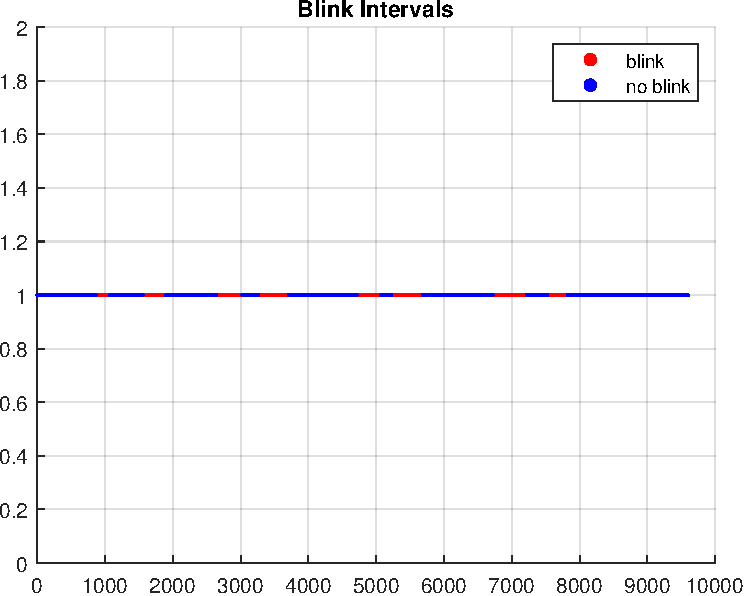
\includegraphics[width=0.5\linewidth]{plot/clean_and_noisy_intervals.pdf}
    \caption{Διαστήματα με και χωρίς θόρυβο στα δεδομένα εκπαίδευσης}
    \label{fig:clean_and_noisy_intervals}
\end{figure}

Στα δεδομένα εκπαίδευσης, γνωρίζουμε εκ των προτέρων τις χρονικές στιγμές όπου στις μετρήσεις μας υπάρχει
θόρυβος, οι οποίες είναι κοινές για όλα τα κανάλια. Μάλιστα, από το Σχήμα~\ref{fig:clean_and_noisy_intervals}
παρατηρούμε ότι αυτές οι χρονικές στιγμές διαμορφώνουν διαστήματα. Έστω 
\[
Q = \{k = 0,...,n-1:\quad \mathbf{y}[k] = \mathbf{v}[k]\} = \underset{j}{{\bigcup}} Q_j
\]
με $Q_j$ το $j$-οστό διάστημα όπου $\mathbf{y}[k] = \mathbf{v}[k]$ και
\[
P = \{k = 0,...,n-1:\quad \mathbf{y}[k] = \mathbf{d}[k] + \mathbf{v}[k]\} = \underset{j}{{\bigcup}} P_j
\]
με $P_j$ το $j$-οστό διάστημα όπου $\mathbf{y}[k] = \mathbf{d}[k] + \mathbf{v}[k]$. 

Θα εκτιμήσουμε τον πίνακα $\mathbf{R}_{vv}^{(i)}$ από τα δεδομένα απουσίας θορύβου, $Q$. 
Ο $\mathbf{R}_{yy}^{(i)}$ προκύπτει αντίστοιχα από τα δεδομένα παρουσίας θορύβου, $P$.

Θεωρώντας ότι η χρονοσειρά $\mathbf{y}_i$ είναι \textit{στάσιμη} σε καθένα από τα διαστήματα $Q_j$, ο πίνακας
αυτοσυσχέτισης $\mathbf{R}_{vv}^{(i,j)}$ του $i$-οστού καναλιού στο $j$-οστό διάστημα όπου απουσιάζει ο 
θόρυβος είναι:
\[
    \mathbf{R}_{vv}^{(i,j)} = 
    \begin{bmatrix}
    r_v^{(i,j)}[0] & r_v^{(i,j)}[1] & \cdots & r_v^{(i,j)}[L-1] \\
    r_v^{(i,j)}[1] & r_v^{(i,j)}[0] & \cdots & r_v^{(i,j)}[L-2] \\
    \vdots & \vdots & \ddots & \vdots \\
    r_v^{(i,j)}[L-1] & r_v^{(i,j)}[L-2] & \cdots & r_v^{(i,j)}[0]
    \end{bmatrix}
\]
όπου $r_v^{(i,j)}[\tau] = \mathbb{E}[v_i[n]v_i[n + \tau]], \quad n,\ldots, n + \tau \in Q_j$ η συνάρτηση 
αυτοσυσχέτισης του $\mathbf{v}_i$ στο διάστημα $Q_j$ και $L$ η μέγιστη υστέρηση. Προφανώς η μέγιστη υστέρηση 
θα πρέπει να είναι μικρότερη από το μικρότερο μέγεθος του διαστήματος με ή χωρίς θόρυβο, 
$L \leq \min\{\underset{j}{\min}|Q_j|, \, \underset{j}{\min}|P_j|\}$.

Είναι σημαντικό να τονίσουμε σε αυτό το σημείο ότι η συνάρτηση αυτοσυσχέτισης και συνακόλουθα ο πίνακας
αυτοσυσχέτισης λαμβάνει υπ' όψιν της μόνο γραμμικές συσχετίσεις. Συνεπώς το φίλτρο 
\selectlanguage{english}Wiener\selectlanguage{greek} βασίζεται στην υπόθεση της γραμμικής αυτοσυσχέτισης
και δεν λαμβάνει υπ' όψιν μη γραμμικές συσχετίσεις μεταξύ των δεδομένων της χρονοσειράς.

Ο πίνακας αυτοσυσχέτισης $R_{vv}^{(i)}$ προκύπτει από τον σταθμισμένο μέσο όρο όλων των $R_{vv}^{(i,j)}$ 
ως εξής:
\[
\mathbf{R}_{vv}^{(i)} = \frac{1}{|Q|}\sum_{j}|Q_j|R_{vv}^{(i,j)}, \quad i=1,\ldots,N
\]

Εργαζόμενοι κατ' αντίστοιχο τρόπο για τα δεδομένα παρουσία θορύβου έχουμε:
\[
\mathbf{R}_{yy}^{(i)} = \frac{1}{|P|}\sum_{j}|P_j|\mathbf{R}_{yy}^{(i,j)}, \quad i=1,\ldots,N
\]

Ο πίνακας \selectlanguage{english}Wiener\selectlanguage{greek} για το $i$-οστό κανάλι θα είναι:
\[
\mathbf{W}^{(i)} = \mathbf{R}_{vv}^{(i)}\left(\mathbf{R}_{yy}^{(i)}\right)^{-1} \in \mathbb{R}^{L \times L}
\]
Το φίλτρο εφαρμόζεται διαδοχικά στις μετρήσεις του εκάστοτε καναλιού σε παράθυρα μήκους $L$ σύμφωνα με την
σχέση:
\[
\hat{\mathbf{v}}_i[k:k+L-1] = \mathbf{W}^{(i)}\mathbf{y}_i[k:k+L-1], \quad i = 1,\ldots,N.
\] 
Είναι προφανές ότι για την εκτίμηση του $\mathbf{v}_i$ χρησιμοποιούνται κάθε φορά οι τελευταίες $L$
μετρήσεις του $\mathbf{y}_i$.

Στο Σχήμα~\ref{fig:single_channel_smoothing} φαίνεται η εφαρμογή του φίλτρου στα δεδομένα εκπαίδευσης 
(αριστερά) και στα δεδομένα ελέγχου (δεξιά) για το κανάλι 1. Παρατηρούμε ότι στα δεδομένα εκπαίδευσης η
εξομάλυνση των μετρήσεων όπου υπάρχει θόρυβος (διαστήματα με μεγάλες διακυμάνσεις) είναι επιτυχής με
κόστος ωστόσο την αλοίωση της πληροφοριάς στα διαστήματα όπου δεν υπάρχει θόρυβος. Επίσης, βλέπουμε ότι
στα δεδομένα ελέγχου το φίλτρο αδυνατεί να επιτύχει την αποθορυβοποίηση του σήματος όταν παρουσιάζονται
μεγάλα \selectlanguage{english}spikes\selectlanguage{greek} του δυναμικού $> 200 V$. Αυτό εξηγείται από
το γεγονός ότι το \selectlanguage{english}Wiener\selectlanguage{greek} φίλτρο βασίζεται σε στατιστικά 
χαρακτηριστικά που υπολογίζονται από τα δεδομένα εκπαίδευσης, όπου τέτοιες ακραίες τιμές δεν εμφανίζονται. 
Τα \selectlanguage{english}spikes\selectlanguage{greek} είναι μη-γραμμικά και υψηλής 
ενέργειας γεγονότα που παραβιάζουν τις υποθέσεις στάσιμης και γραμμικής συσχέτισης πάνω στις οποίες 
βασίζεται το φίλτρο, με αποτέλεσμα την αδυναμία του να τα εξομαλύνει επαρκώς.

\begin{figure}[htbp]
    \centering
    \begin{subfigure}[b]{0.45\textwidth}
        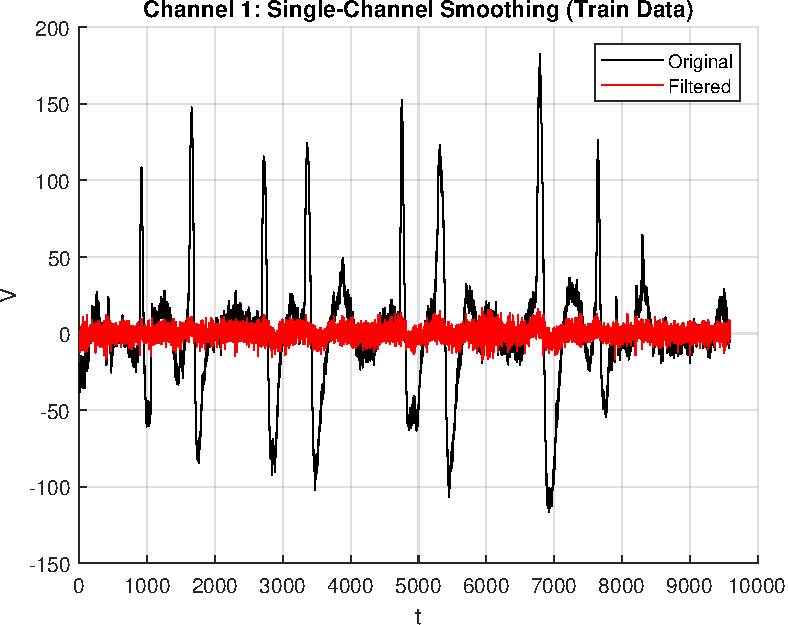
\includegraphics[width=\textwidth]{plot/single_channel_smoothing_train.pdf}
        \caption{}
        \label{fig:single_channel_smoothing_train}
    \end{subfigure}
    \hfill
    \begin{subfigure}[b]{0.45\textwidth}
        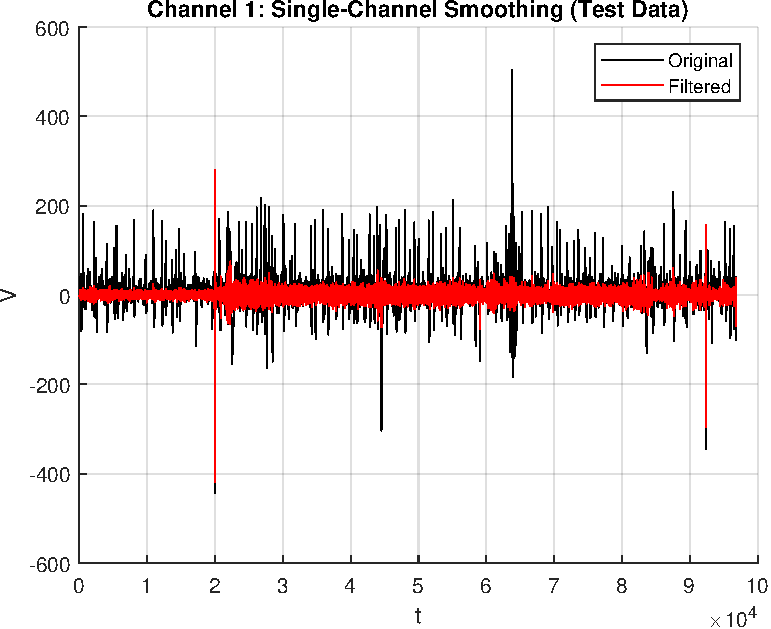
\includegraphics[width=\textwidth]{plot/single_channel_smoothing_test.pdf}
        \caption{}
        \label{fig:single_channel_smoothing_test}
    \end{subfigure}

    \caption{Εφαρμογή μονοκαναλικού \selectlanguage{english}Smoothing Wiener Filter\selectlanguage{greek} 
    στα α) δεδομένα εκπαίδευσης β) δεδομένα ελέγχου}
    \label{fig:single_channel_smoothing}
\end{figure}

\section*{Πολυκαναλικό \selectlanguage{english}Wiener Smoothing\selectlanguage{greek}}
Μέχρι στιγμής στην ανάλυσή μας εξετάζαμε κάθε κανάλι μεμονωμένα, αγνοήσαμε δηλαδή τη συσχέτιση που υπάρχει
μεταξύ των μετρήσεών τους. Αυτό ωστόσο δεν είναι απόλυτα σωστό, καθώς ο θόρυβος είναι εντονότερος στα μετωπιαία
ηλεκτρόδια, επομένως υπάρχει συσχέτιση μεταξύ των μετρήσεων των διαφορετικών καναλιών. Σε αυτή την ενότητα θα
συμπεριλάβουμε αυτές τις συσχετίσεις μεταξύ των καναλιών.

Έστω $\mathbf{Y}_t^{(j)} \in \mathbb{R}^{N\cdot L}$ το διάνυσμα στήλη που περιέχει τις τιμές όλων των καναλιών
στοιβαγμένες για χρονικό παράθυρο μήκους $L$, τη χρονική στιγμή $t$ με $t,\ldots, t+L-1 \in P_j$:
\[
\mathbf{Y}_t = 
\begin{bmatrix}
    \mathbf{y}_1[t:t+L-1] \\
    \mathbf{y}_2[t:t+L-1] \\
    \vdots \\
    \mathbf{y}_N[t:t+L-1] \\
\end{bmatrix}
\]
όπου $\mathbf{y}_i[t:t+L-1] \in \mathbb{R}^L$ οι μετρήσεις του $i$-οστού καναλιού. Χωρίς βλάβη της γενικότητας
θεωρούμε ότι το διάστημα $P_j$ ξεκινάει από την στιγμή $t=1$. Σχηματίζουμε τον πίνακα 
$\mathbf{Y}^{(j)} = [\mathbf{Y}_1^{(j)} \quad \mathbf{Y}_2^{(j)} \quad \cdots \quad \mathbf{Y}_N^{(j)}] 
\in \mathbb{R}^{N \cdot L \times T}, \quad T = |P_j| - L + 1$:
\[
\mathbf{Y}^{(j)} = 
\begin{bmatrix}
    \mathbf{y}_1[1:L] & \mathbf{y}_1[2:L+1] & \cdots & \mathbf{y}_1[n-L+1:n] \\
    \mathbf{y}_2[1:L] & \mathbf{y}_2[2:L+1] & \cdots & \mathbf{y}_2[n-L+1:n] \\
    \vdots & \vdots & \ddots & \vdots \\
    \mathbf{y}_N[1:L] & \mathbf{y}_N[2:L+1] & \cdots & \mathbf{y}_N[n-L+1:n]
\end{bmatrix}
\]
Αν υποθέσουμε ότι $\mathbb{E}[\mathbf{Y}_t^{(j)}] = 0, \, t=1,\ldots,L$, τότε ο πίνακας συσχέτισης 
$\mathbf{R}_{yy}^{(j)}$ για το διάστημα $P_j$ θα δίνεται από:
\[
\mathbf{R}_{yy}^{(j)} = 
\frac{1}{T} \sum_{i=1}^T \mathbf{Y}_i^{(j)} \left(\mathbf{Y}_i^{(j)}\right)^{\top} = 
\frac{1}{T} \mathbf{Y}^{(j)} \cdot \left(\mathbf{Y}^{(j)}\right)^{\top} = 
\]
Αν επιπλέον οι χρονοσειρές δύο καναλιών $p,\,q$ είναι από κοινού στάσιμες 
$\mathbb{E}[\mathbf{y}_p[k] \cdot \mathbf{y}_q[l]] = r_{pq}[k-l] \in \mathbb{R}$, δηλαδή η 
εταιροσυσχέτισή τους εξαρτάται μόνο από την υστέρηση $\tau = k - l$ και όχι από τον χρόνο, τότε:
\[
\mathbf{R}_{yy}^{(j)} =
\begin{bmatrix}
    \mathbf{R}_{11} & \mathbf{R}_{12} & \cdots & \mathbf{R}_{1N} \\
    \mathbf{R}_{21} & \mathbf{R}_{22} & \cdots & \mathbf{R}_{2N} \\
    \vdots & \vdots & \ddots & \vdots \\
    \mathbf{R}_{N1} & \mathbf{R}_{N2} & \cdots & \mathbf{R}_{NN}
\end{bmatrix}
\]
όπου $\mathbf{R}_{pq} \in \mathbb{R}^{L \times L}$ ο πίνακας συνδιασποράς μεταξύ των καναλιών $p$ και $q$
για υστερήσεις $\tau = 0,\ldots,L-1$. Το στοιχείο $[\mathbf{R}_{pq}]_{k,l} = r_{pq}[k-l]$ δείχνει πόσο 
συσχετίζεται η τιμή του καναλιού $p$ για υστέρηση $k-1$ με την τιμή του καναλιού $q$ για υστέρηση $l-1$.

Όπως και στην μονοκαναλική προσέγγιση, ο πίνακας $\mathbf{R}_{yy}$ δίνεται από τον σταθμισμένο μέσο όρο 
των πινάκων διασποράς για όλα τα διαστήματα όπου υπάρχει θόρυβος:
\[
\mathbf{R}_{yy} = \frac{1}{|P|} \sum_j |P_j| \mathbf{R}_{yy}^{(j)}
\]
Εργαζόμενοι κατ' αντίστοιχο τρόπο στα διαστήματα $Q_j$ όπου απουσιάζει ο θόρυβος, προκύπτει ο πίνακας 
$\mathbf{R}_{vv}$.

Ο πίνακας \selectlanguage{english}Wiener\selectlanguage{greek} θα είναι:
\[
\mathbf{W} = \mathbf{R}_{vv}\mathbf{R}_{yy}^{-1} \in \mathbb{R}^{N \cdot L \times N \cdot L}
\]
Και εδώ το φίλτρο εφαρμόζεται διαδοχικά σε παράθυρα μήκους $L$ σύμφωνα με την σχέση:
\[
\hat{\mathbf{V}}[k:k+L-1] = \mathbf{W} \cdot \mathbf{Y}[k:k+L-1]
\] 
Είναι προφανές ότι για την εκτίμηση του $\mathbf{v}_i$ χρησιμοποιούνται κάθε φορά οι τελευταίες $L$
μετρήσεις του $\mathbf{y}_i$.

\begin{figure}[htbp]
    \centering
    \begin{subfigure}[b]{0.45\textwidth}
        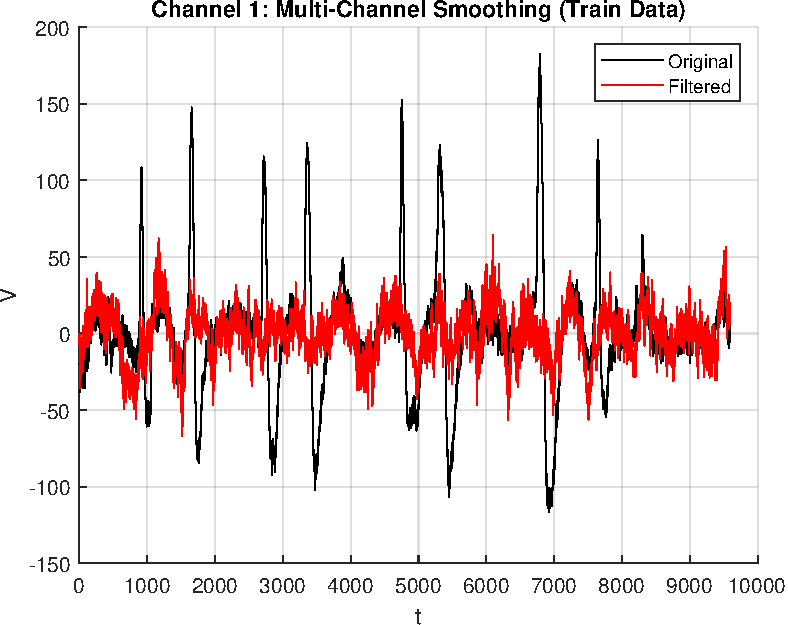
\includegraphics[width=\textwidth]{plot/multi_channel_smoothing_train.pdf}
        \caption{}
        \label{fig:multi_channel_smoothing_train}
    \end{subfigure}
    \hfill
    \begin{subfigure}[b]{0.45\textwidth}
        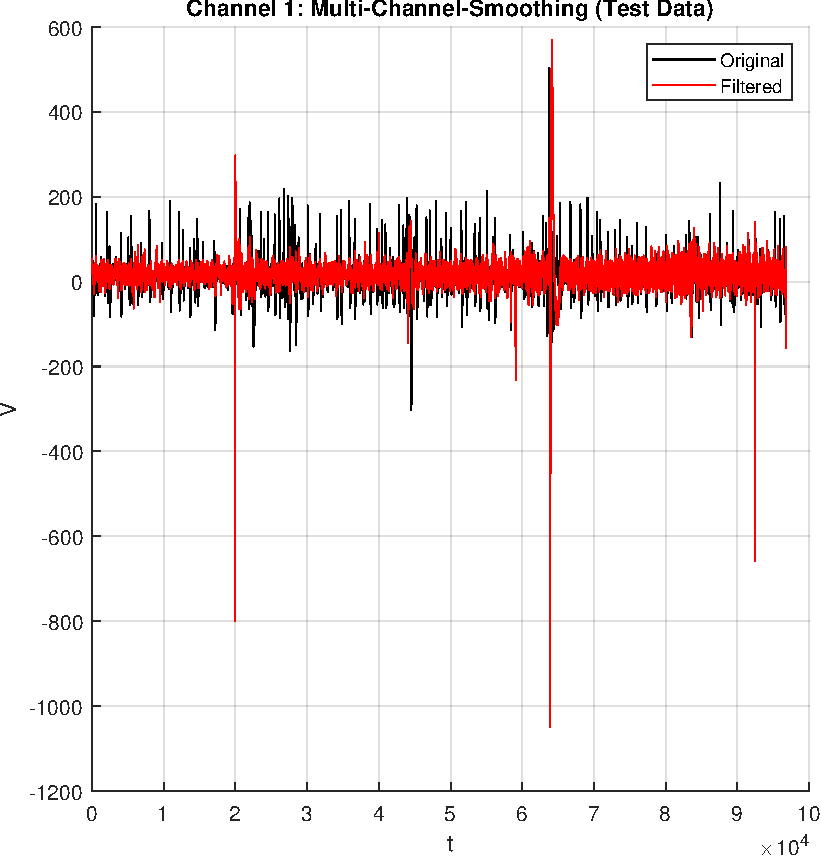
\includegraphics[width=\textwidth]{plot/multi_channel_smoothing_test.pdf}
        \caption{}
        \label{fig:multi_channel_smoothing_test}
    \end{subfigure}

    \caption{Εφαρμογή πολυκαναλικού \selectlanguage{english}Smoothing Wiener Filter\selectlanguage{greek} 
    στα α) δεδομένα εκπαίδευσης β) δεδομένα ελέγχου}
    \label{fig:multi_channel_smoothing}
\end{figure}

\end{document}
